\begin{frame}{Số phức}
    \begin{center}
        \begin{minipage}{0.4\linewidth}
            \resizebox{1\linewidth}{!}{


\tikzset{every picture/.style={line width=0.75pt}} %set default line width to 0.75pt        

\begin{tikzpicture}[x=0.75pt,y=0.75pt,yscale=-1,xscale=1]
%uncomment if require: \path (0,15225); %set diagram left start at 0, and has height of 15225

%Straight Lines [id:da5015611160293443] 
\draw    (526,6086) -- (683.5,6086) ;
\draw [shift={(685.5,6086)}, rotate = 180] [color={rgb, 255:red, 0; green, 0; blue, 0 }  ][line width=0.75]    (10.93,-3.29) .. controls (6.95,-1.4) and (3.31,-0.3) .. (0,0) .. controls (3.31,0.3) and (6.95,1.4) .. (10.93,3.29)   ;
%Straight Lines [id:da7739785169188371] 
\draw    (526,6086) -- (526,5966) ;
\draw [shift={(526,5964)}, rotate = 90] [color={rgb, 255:red, 0; green, 0; blue, 0 }  ][line width=0.75]    (10.93,-3.29) .. controls (6.95,-1.4) and (3.31,-0.3) .. (0,0) .. controls (3.31,0.3) and (6.95,1.4) .. (10.93,3.29)   ;
%Straight Lines [id:da38078718023855684] 
\draw  [dash pattern={on 0.84pt off 2.51pt}]  (526,6033) -- (608.5,6033) ;
\draw [shift={(608.5,6033)}, rotate = 0] [color={rgb, 255:red, 0; green, 0; blue, 0 }  ][fill={rgb, 255:red, 0; green, 0; blue, 0 }  ][line width=0.75]      (0, 0) circle [x radius= 3.35, y radius= 3.35]   ;
%Straight Lines [id:da36972469805515473] 
\draw  [dash pattern={on 0.84pt off 2.51pt}]  (608.5,6033) -- (608.5,6086) ;

% Text Node
\draw (474,5948) node [anchor=north west][inner sep=0.75pt]    {$Im( z)$};
% Text Node
\draw (615,6008) node [anchor=north west][inner sep=0.75pt]    {$z\ =\ a\ +\ ib$};
% Text Node
\draw (682,6092) node [anchor=north west][inner sep=0.75pt]    {$Re( z)$};
% Text Node
\draw (601,6091) node [anchor=north west][inner sep=0.75pt]    {$a$};
% Text Node
\draw (505,6022) node [anchor=north west][inner sep=0.75pt]    {$b$};
% Text Node
\draw (507,6083) node [anchor=north west][inner sep=0.75pt]    {$O$};


\end{tikzpicture}}
        \end{minipage}
        \hspace{2mm}
        \begin{minipage}{0.4\linewidth}
            Số ảo \(\mathbf{i}\) được định nghĩa \cite{gilbert2009introduction}
            \begin{equation}
                i = \sqrt{-1}.
                \label{eq:1.1_1}
            \end{equation}
            Không gian số phức là 
            \begin{equation*}
                \mathcal{C} = (a,b) | a,b \in \mathcal{R}
            \end{equation*}
        \end{minipage}
    \end{center}
\end{frame}

\begin{frame}{Công thức euler}
    \begin{mdframed}[backgroundcolor=BlueDefault!10, linecolor=BlueDefault, linewidth=0.5pt, roundcorner=1pt]
        Công thức euler gọi là phép quay một góc \(\theta\) trong mặt phẳng phức.
        \begin{equation}
            e^{i\theta} = \cos{\theta} + i \sin{\theta}
            \label{eq:1.1_2}
        \end{equation}
    \end{mdframed}
    \vspace{2mm}
    
    Ví dụ: áp dụng phép quay \(\theta\) cho số phức \(z = a + i b\)
    \begin{center}
        \begin{minipage}{0.4\linewidth}
            \begin{equation*}
            \begin{split}
                z' &= \left[\begin{array}{cc}
               \cos{\theta}  & -\sin{\theta} \\
               \sin{\theta}  & \cos{\theta}
            \end{array} \right] \left[
            \begin{array}{c}
                a \\
                b
            \end{array}
            \right]  \\
            &= (a + i b) e^{i\theta}
            \end{split}
            \end{equation*}
        \end{minipage}
        \hspace{1mm}
        \begin{minipage}{0.4\linewidth}
            \begin{center}
                \resizebox{1\linewidth}{!}{


\tikzset{every picture/.style={line width=0.75pt}} %set default line width to 0.75pt        

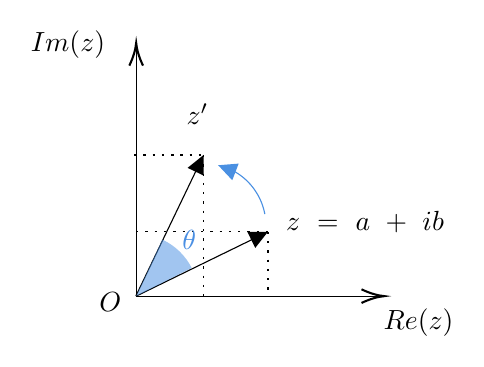
\begin{tikzpicture}[x=0.75pt,y=0.75pt,yscale=-1,xscale=1]
%uncomment if require: \path (0,15225); %set diagram left start at 0, and has height of 15225

%Straight Lines [id:da5015611160293443] 
\draw    (526,6086) -- (643.5,6086) ;
\draw [shift={(645.5,6086)}, rotate = 180] [color={rgb, 255:red, 0; green, 0; blue, 0 }  ][line width=0.75]    (10.93,-3.29) .. controls (6.95,-1.4) and (3.31,-0.3) .. (0,0) .. controls (3.31,0.3) and (6.95,1.4) .. (10.93,3.29)   ;
%Straight Lines [id:da7739785169188371] 
\draw    (526,6086) -- (526,5966) ;
\draw [shift={(526,5964)}, rotate = 90] [color={rgb, 255:red, 0; green, 0; blue, 0 }  ][line width=0.75]    (10.93,-3.29) .. controls (6.95,-1.4) and (3.31,-0.3) .. (0,0) .. controls (3.31,0.3) and (6.95,1.4) .. (10.93,3.29)   ;
%Straight Lines [id:da6097015977657645] 
\draw  [dash pattern={on 0.84pt off 2.51pt}]  (526,6055) -- (589.5,6055) ;
%Straight Lines [id:da06830863122513897] 
\draw  [dash pattern={on 0.84pt off 2.51pt}]  (589.5,6055) -- (589.5,6086) ;
%Straight Lines [id:da1339436079722769] 
\draw    (526,6086) -- (586.8,6056.32) ;
\draw [shift={(589.5,6055)}, rotate = 153.98] [fill={rgb, 255:red, 0; green, 0; blue, 0 }  ][line width=0.08]  [draw opacity=0] (8.93,-4.29) -- (0,0) -- (8.93,4.29) -- cycle    ;
%Straight Lines [id:da12876867450395124] 
\draw    (525.83,6086) -- (557.2,6020.7) ;
\draw [shift={(558.5,6018)}, rotate = 115.66] [fill={rgb, 255:red, 0; green, 0; blue, 0 }  ][line width=0.08]  [draw opacity=0] (8.93,-4.29) -- (0,0) -- (8.93,4.29) -- cycle    ;
%Straight Lines [id:da6964942743081263] 
\draw  [dash pattern={on 0.84pt off 2.51pt}]  (525,6018) -- (558.5,6018) ;
%Straight Lines [id:da21207065554446136] 
\draw  [dash pattern={on 0.84pt off 2.51pt}]  (558.5,6018) -- (558.5,6086) ;
%Straight Lines [id:da7448312272789616] 
\draw [color={rgb, 255:red, 74; green, 144; blue, 226 }  ,draw opacity=1 ]   (573.49,6026.01) -- (568.31,6024.02) ;
\draw [shift={(565.51,6022.94)}, rotate = 21.06] [fill={rgb, 255:red, 74; green, 144; blue, 226 }  ,fill opacity=1 ][line width=0.08]  [draw opacity=0] (8.93,-4.29) -- (0,0) -- (8.93,4.29) -- cycle    ;
%Shape: Arc [id:dp7227532122430883] 
\draw  [draw opacity=0] (573.49,6026.01) .. controls (580.94,6030.31) and (586.36,6037.72) .. (587.99,6046.47) -- (558.5,6052) -- cycle ; \draw  [color={rgb, 255:red, 74; green, 144; blue, 226 }  ,draw opacity=1 ] (573.49,6026.01) .. controls (580.94,6030.31) and (586.36,6037.72) .. (587.99,6046.47) ;  
%Shape: Arc [id:dp5675882433264926] 
\draw  [draw opacity=0][fill={rgb, 255:red, 74; green, 144; blue, 226 }  ,fill opacity=0.52 ] (538.61,6058.77) .. controls (544.71,6061.6) and (549.7,6066.42) .. (552.75,6072.4) -- (526,6086) -- cycle ; \draw  [draw opacity=0] (538.61,6058.77) .. controls (544.71,6061.6) and (549.7,6066.42) .. (552.75,6072.4) ;  

% Text Node
\draw (474,5957) node [anchor=north west][inner sep=0.75pt]    {$Im( z)$};
% Text Node
\draw (597,6044) node [anchor=north west][inner sep=0.75pt]    {$z\ =\ a\ +\ ib$};
% Text Node
\draw (644,6091) node [anchor=north west][inner sep=0.75pt]    {$Re( z)$};
% Text Node
\draw (507,6083) node [anchor=north west][inner sep=0.75pt]    {$O$};
% Text Node
\draw (549,5992) node [anchor=north west][inner sep=0.75pt]    {$z'$};
% Text Node
\draw (547,6053) node [anchor=north west][inner sep=0.75pt]    {$\textcolor[rgb]{0.29,0.56,0.89}{\theta }$};


\end{tikzpicture}}
            \end{center}
        \end{minipage}
    \end{center}
\end{frame}
\begin{frame}{Số phức}
    \begin{mdframed}[backgroundcolor=BlueDefault!10, linecolor=BlueDefault, linewidth=0.5pt, roundcorner=1pt]
        Công thức euler còn là cách biểu diễn khác của số phức.
        \begin{equation}
            z = |z| e^{i\theta} = |z|(\cos{\theta} + i \sin{\theta})
            \label{eq:1.1_3}
        \end{equation}
        Với \(|z|\) là module của số phức \(z\), \(\theta\) là góc lệch của so với trục thực.
    \end{mdframed}
    \begin{center}
        \begin{minipage}{0.4\linewidth}
        \resizebox{1\linewidth}{!}{


\tikzset{every picture/.style={line width=0.75pt}} %set default line width to 0.75pt        

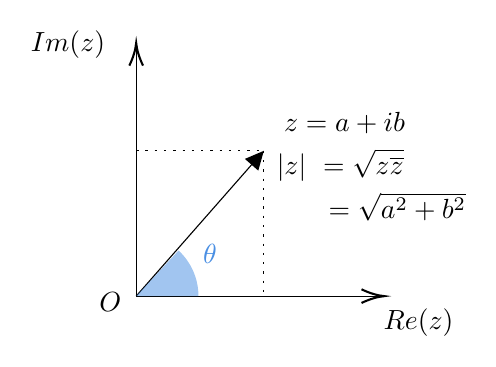
\begin{tikzpicture}[x=0.75pt,y=0.75pt,yscale=-1,xscale=1]
%uncomment if require: \path (0,15225); %set diagram left start at 0, and has height of 15225

%Straight Lines [id:da5597477618794069] 
\draw    (843,6091) -- (960.5,6091) ;
\draw [shift={(962.5,6091)}, rotate = 180] [color={rgb, 255:red, 0; green, 0; blue, 0 }  ][line width=0.75]    (10.93,-3.29) .. controls (6.95,-1.4) and (3.31,-0.3) .. (0,0) .. controls (3.31,0.3) and (6.95,1.4) .. (10.93,3.29)   ;
%Straight Lines [id:da12681955407125622] 
\draw    (843,6091) -- (843,5971) ;
\draw [shift={(843,5969)}, rotate = 90] [color={rgb, 255:red, 0; green, 0; blue, 0 }  ][line width=0.75]    (10.93,-3.29) .. controls (6.95,-1.4) and (3.31,-0.3) .. (0,0) .. controls (3.31,0.3) and (6.95,1.4) .. (10.93,3.29)   ;
%Straight Lines [id:da8100573273316289] 
\draw  [dash pattern={on 0.84pt off 2.51pt}]  (843,6021) -- (904.5,6021) ;
%Straight Lines [id:da18835817233889307] 
\draw  [dash pattern={on 0.84pt off 2.51pt}]  (904.5,6021) -- (904.5,6091) ;
%Straight Lines [id:da16390059449403382] 
\draw    (843,6091) -- (902.52,6023.25) ;
\draw [shift={(904.5,6021)}, rotate = 131.3] [fill={rgb, 255:red, 0; green, 0; blue, 0 }  ][line width=0.08]  [draw opacity=0] (8.93,-4.29) -- (0,0) -- (8.93,4.29) -- cycle    ;
%Shape: Arc [id:dp60111373870411] 
\draw  [draw opacity=0][fill={rgb, 255:red, 74; green, 144; blue, 226 }  ,fill opacity=0.52 ] (863.41,6069.02) .. controls (869.31,6074.49) and (873,6082.32) .. (873,6091) -- (843,6091) -- cycle ; \draw  [draw opacity=0] (863.41,6069.02) .. controls (869.31,6074.49) and (873,6082.32) .. (873,6091) ;  

% Text Node
\draw (791,5962) node [anchor=north west][inner sep=0.75pt]    {$Im( z)$};
% Text Node
\draw (913,6001) node [anchor=north west][inner sep=0.75pt]    {$z = a + ib$};
% Text Node
\draw (961,6096) node [anchor=north west][inner sep=0.75pt]    {$Re( z)$};
% Text Node
\draw (824,6088) node [anchor=north west][inner sep=0.75pt]    {$O$};
% Text Node
\draw (909.5,6019) node [anchor=north west][inner sep=0.75pt]    {$|z|\ =\sqrt{z \overline{z}}  $};
\draw (934.5,6040) node [anchor=north west][inner sep=0.75pt]    {$= \sqrt{a^2 + b^2} $};
% Text Node
\draw (874,6065) node [anchor=north west][inner sep=0.75pt]    {$\textcolor[rgb]{0.29,0.56,0.89}{\theta }$};


\end{tikzpicture}}
        \end{minipage}
        \hspace{3mm}
        \begin{minipage}{0.35\linewidth}
        Liên hợp phức: 
        \begin{equation}
            z = a + ib \rightarrow \overline{z} = a - ib.
            \label{eq:1.1_4}
        \end{equation}
        \end{minipage}
    \end{center}
\end{frame}